
\section{Data Analytics}
\label{sec:Data Analytics}

\subsection{Cluster Analysis}
\label{subsec:clustering}
Firstly, we will create clusters based on trip durations, weather (temperatures and precip) and revenue characteristics as described and calculated in the descriptive section. Thus, we develop station-related clusters and transaction-related clusters. Secondly, we will try to develop clusters of stations based on activity measures (KPI2, number of starting rides per station).
During clustering, we would like to refer to the mean duration of each available hour to one ‘trip’. The application of K-Means as a hard clustering method and the Gaussian Mixture model as soft clustering method results in three reasonable clusters describing duration as a single input feature.  The number of clusters is derived from the elbow point and silhouette scores, visualized in \hyperref[LossKMeans_Duration_dpi300]{Appednix Figure X} and \hyperref[Silhouette_Duration]{Appendix Figure X}. The visualization of the clusters reveals short trips (<14 min.), medium trips (<24 min.) and long trips (>24 min.) (\hyperref[FINAL_Clusters_Duration]{Figure X}). The Gaussian Mixture model result suggests, instead of a cluster for long trips, a cluster for extreme trips, which includes both very short and long trips (\hyperref[FINAL_Cluster_Gaussian_Duration]{Appendix Figure X}). 

\begin{figure}[H]
   \centering
    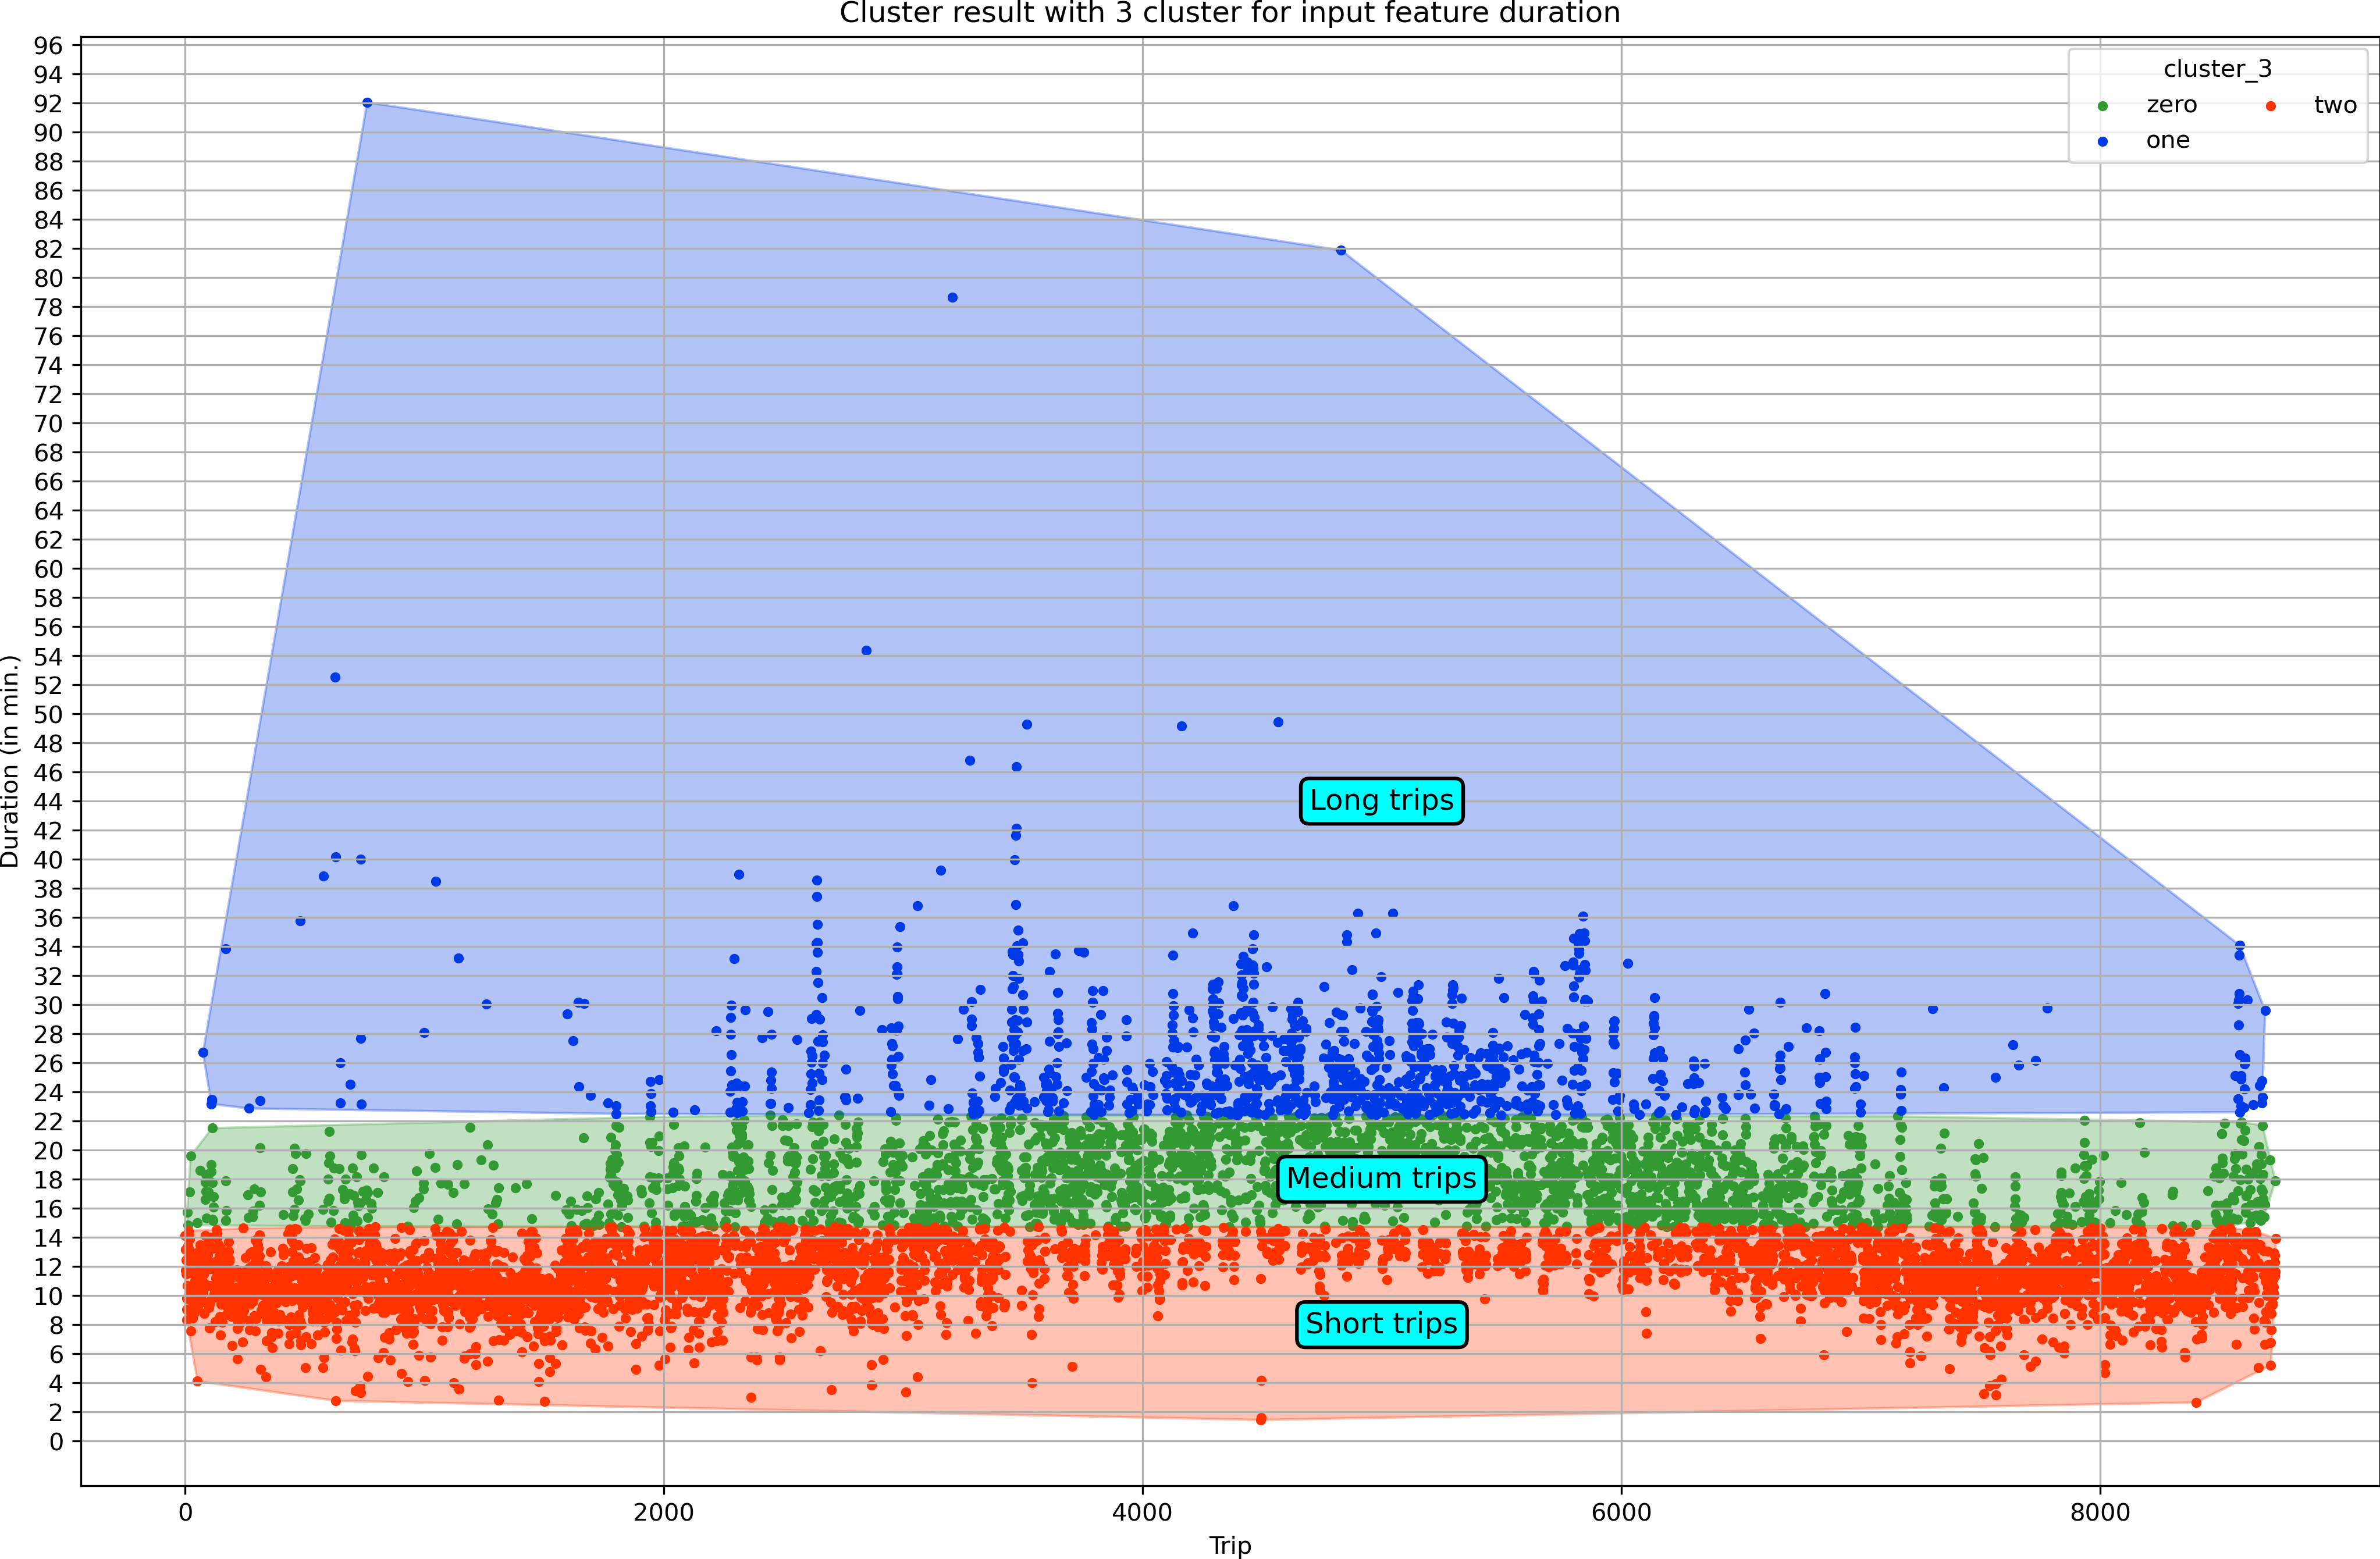
\includegraphics[width=0.75\linewidth]{./Figures/FINAL_Clusters_Duration.png}
    \caption{Cluster result with 3 cluster for input feature duration}
    \label{FINAL_Clusters_Duration}
\end{figure}

The clustering with duration and temperature lead to six differentiations, visualized in \hyperref[FINAL_Cluster_KMEANS_Duration_Temp]{Figure X}. Following the elbow method (\hyperref[Loss_Duration_Temp]{Appendix Figure X}), one would choose the cluster result with 3 clusters (\hyperref[Cluster_KMEANS_Duration_Temp]{Appendix Figure X}), but this cluster assignment seems too superficial and does not represent the different combined intervals of duration and temperature values in an adequate manner. The Gaussian model adds a new perspective, as the data is now largely represented by elliptical cluster structures. The clusters leave a large scope for interpretation and are highly subjective. Despite the better coverage of elliptical structures, a more reasonable classification as with K-Means cannot be found (\hyperref[Silhouette_Gaussian_Duration_Temp]{Appendix Figure X} and \hyperref[Clusters_Gaussian_Duration_Temp]{Appendix Figure X}).

\begin{figure}[H]
   \centering
    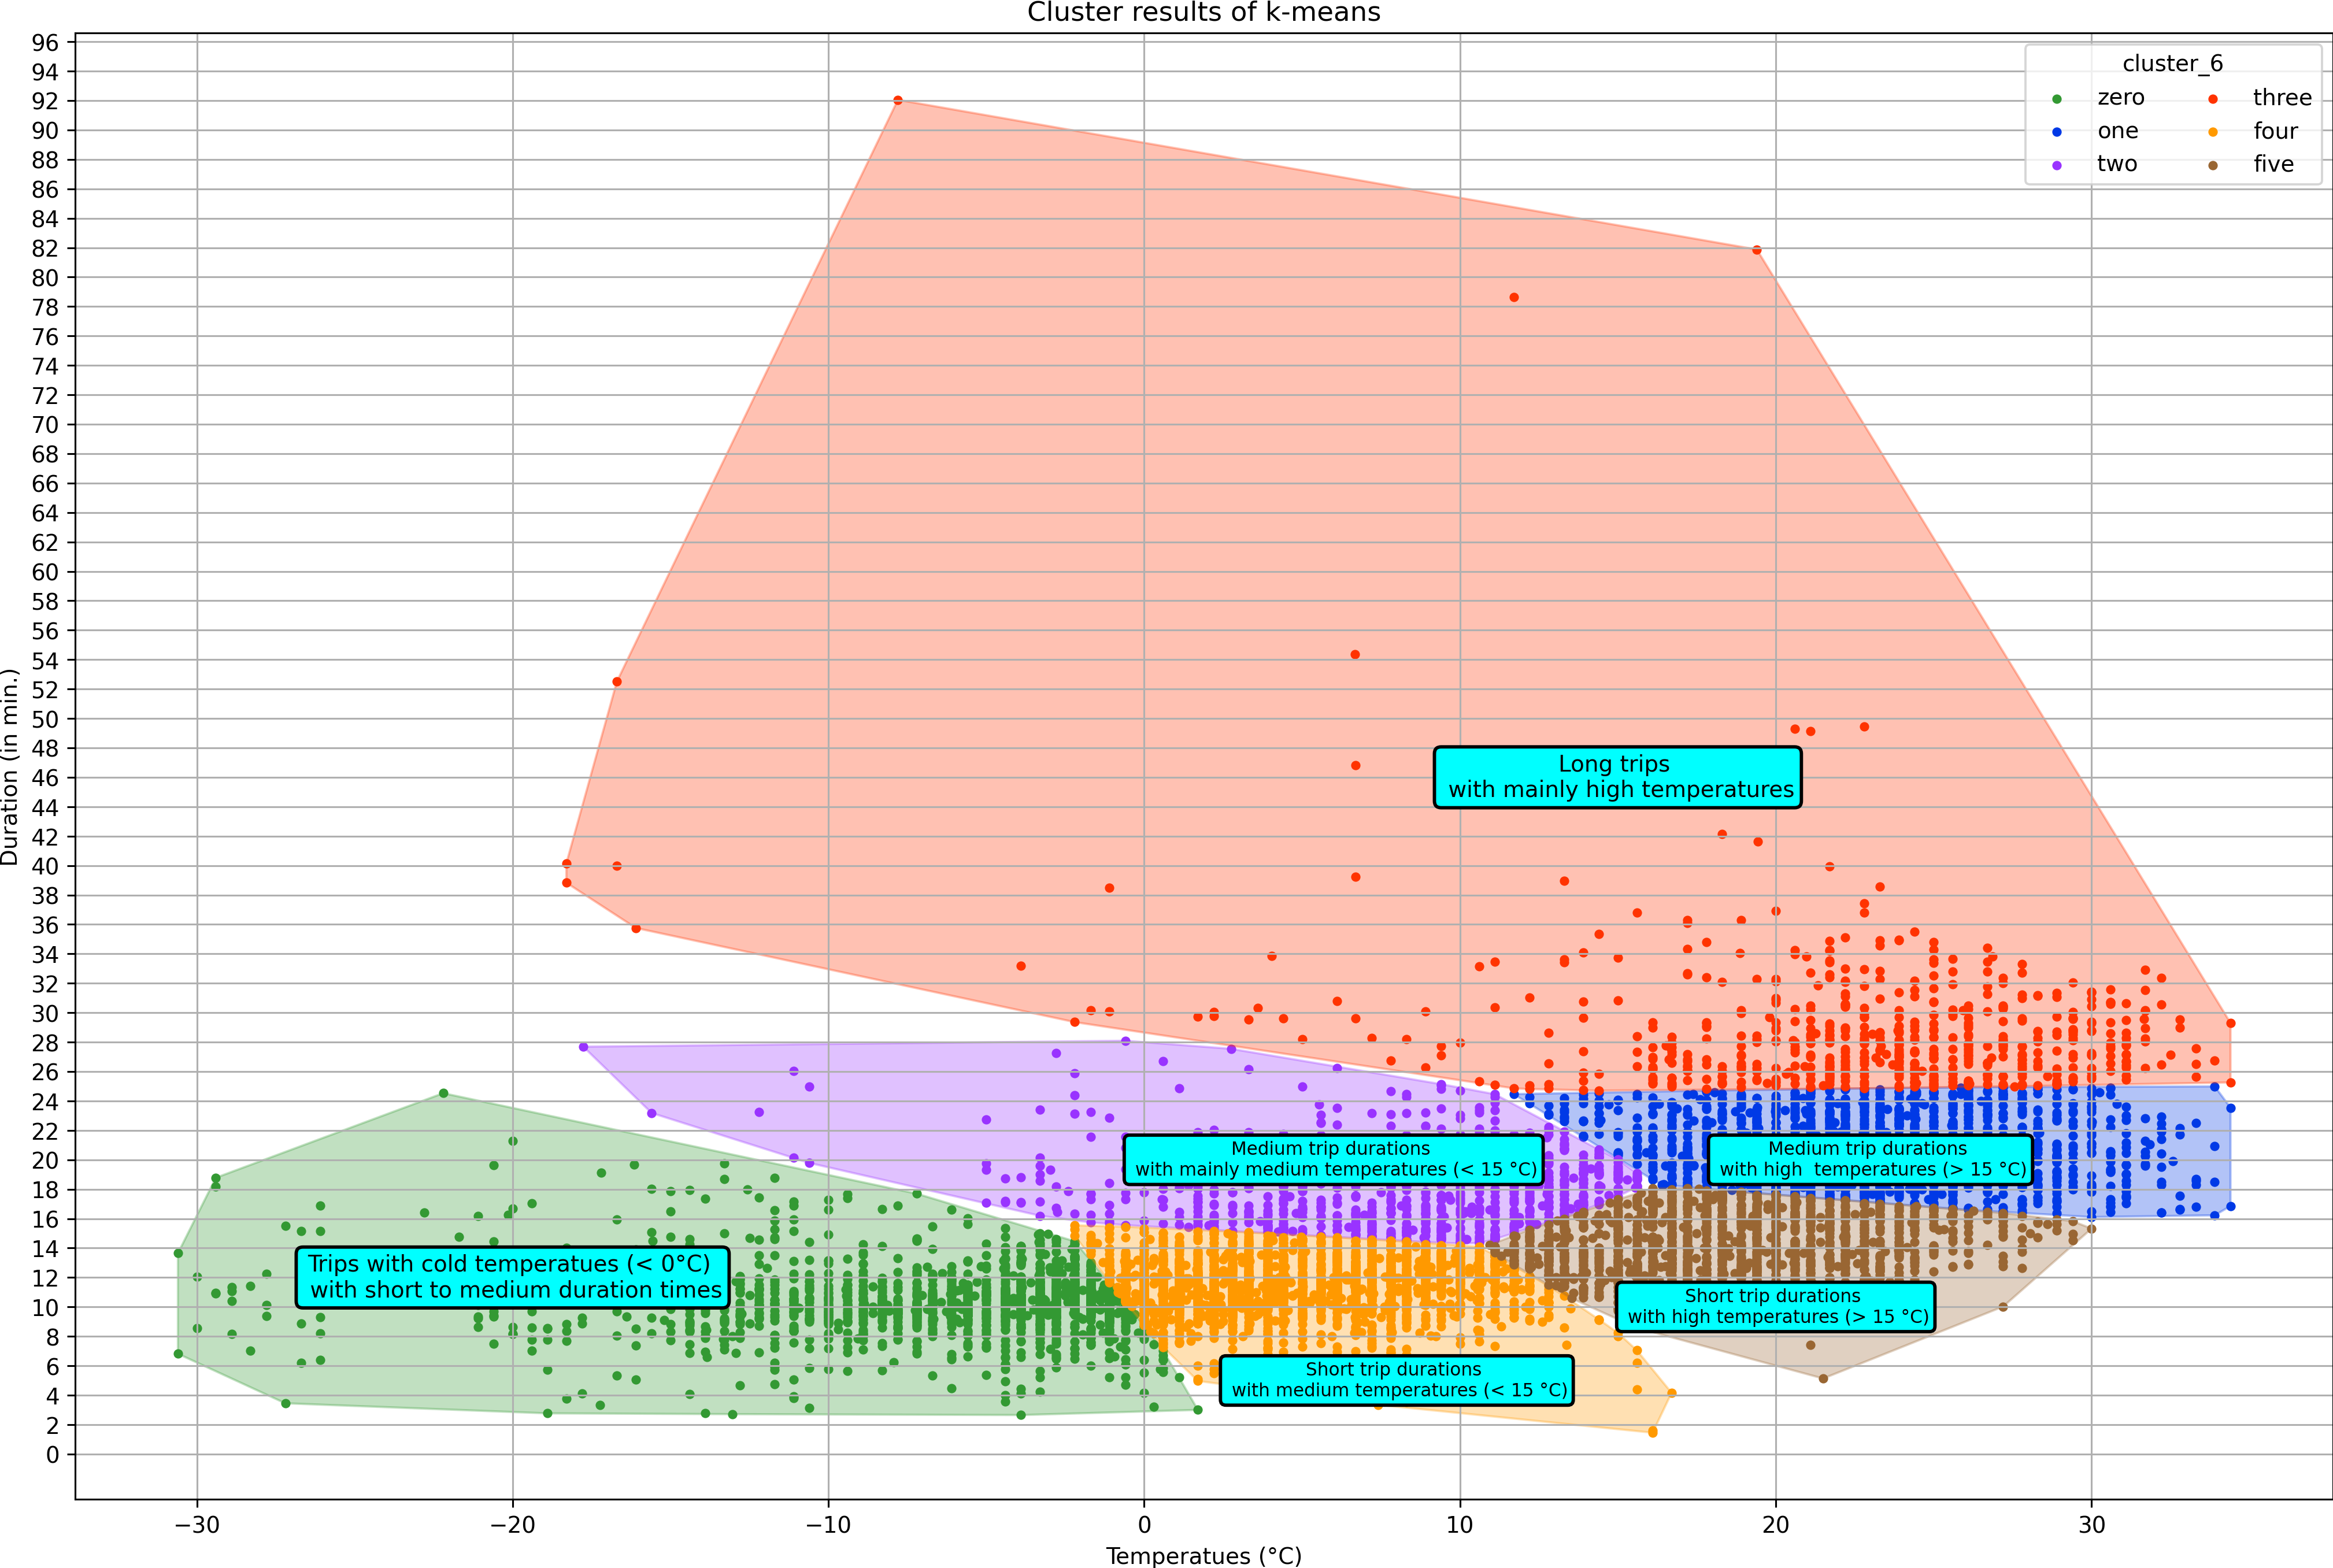
\includegraphics[width=0.8\linewidth]{./Figures/FINAL_Cluster_KMEANS_Duration_Temp.png}
    \caption{Cluster result K-Means}
    \label{FINAL_Cluster_KMEANS_Duration_Temp}
\end{figure}

Taking precip into account, the complementary cluster to the K-Means result with 6 cluster is visualized in \hyperref[FINAL_Cluster_Duration_Temp_Precip]{Figure X}. The K-Means algorithm found the same 6 clusters, but additionally differentiate rain trips by adding two rain clusters.\\

\begin{figure}[H]
   \centering
    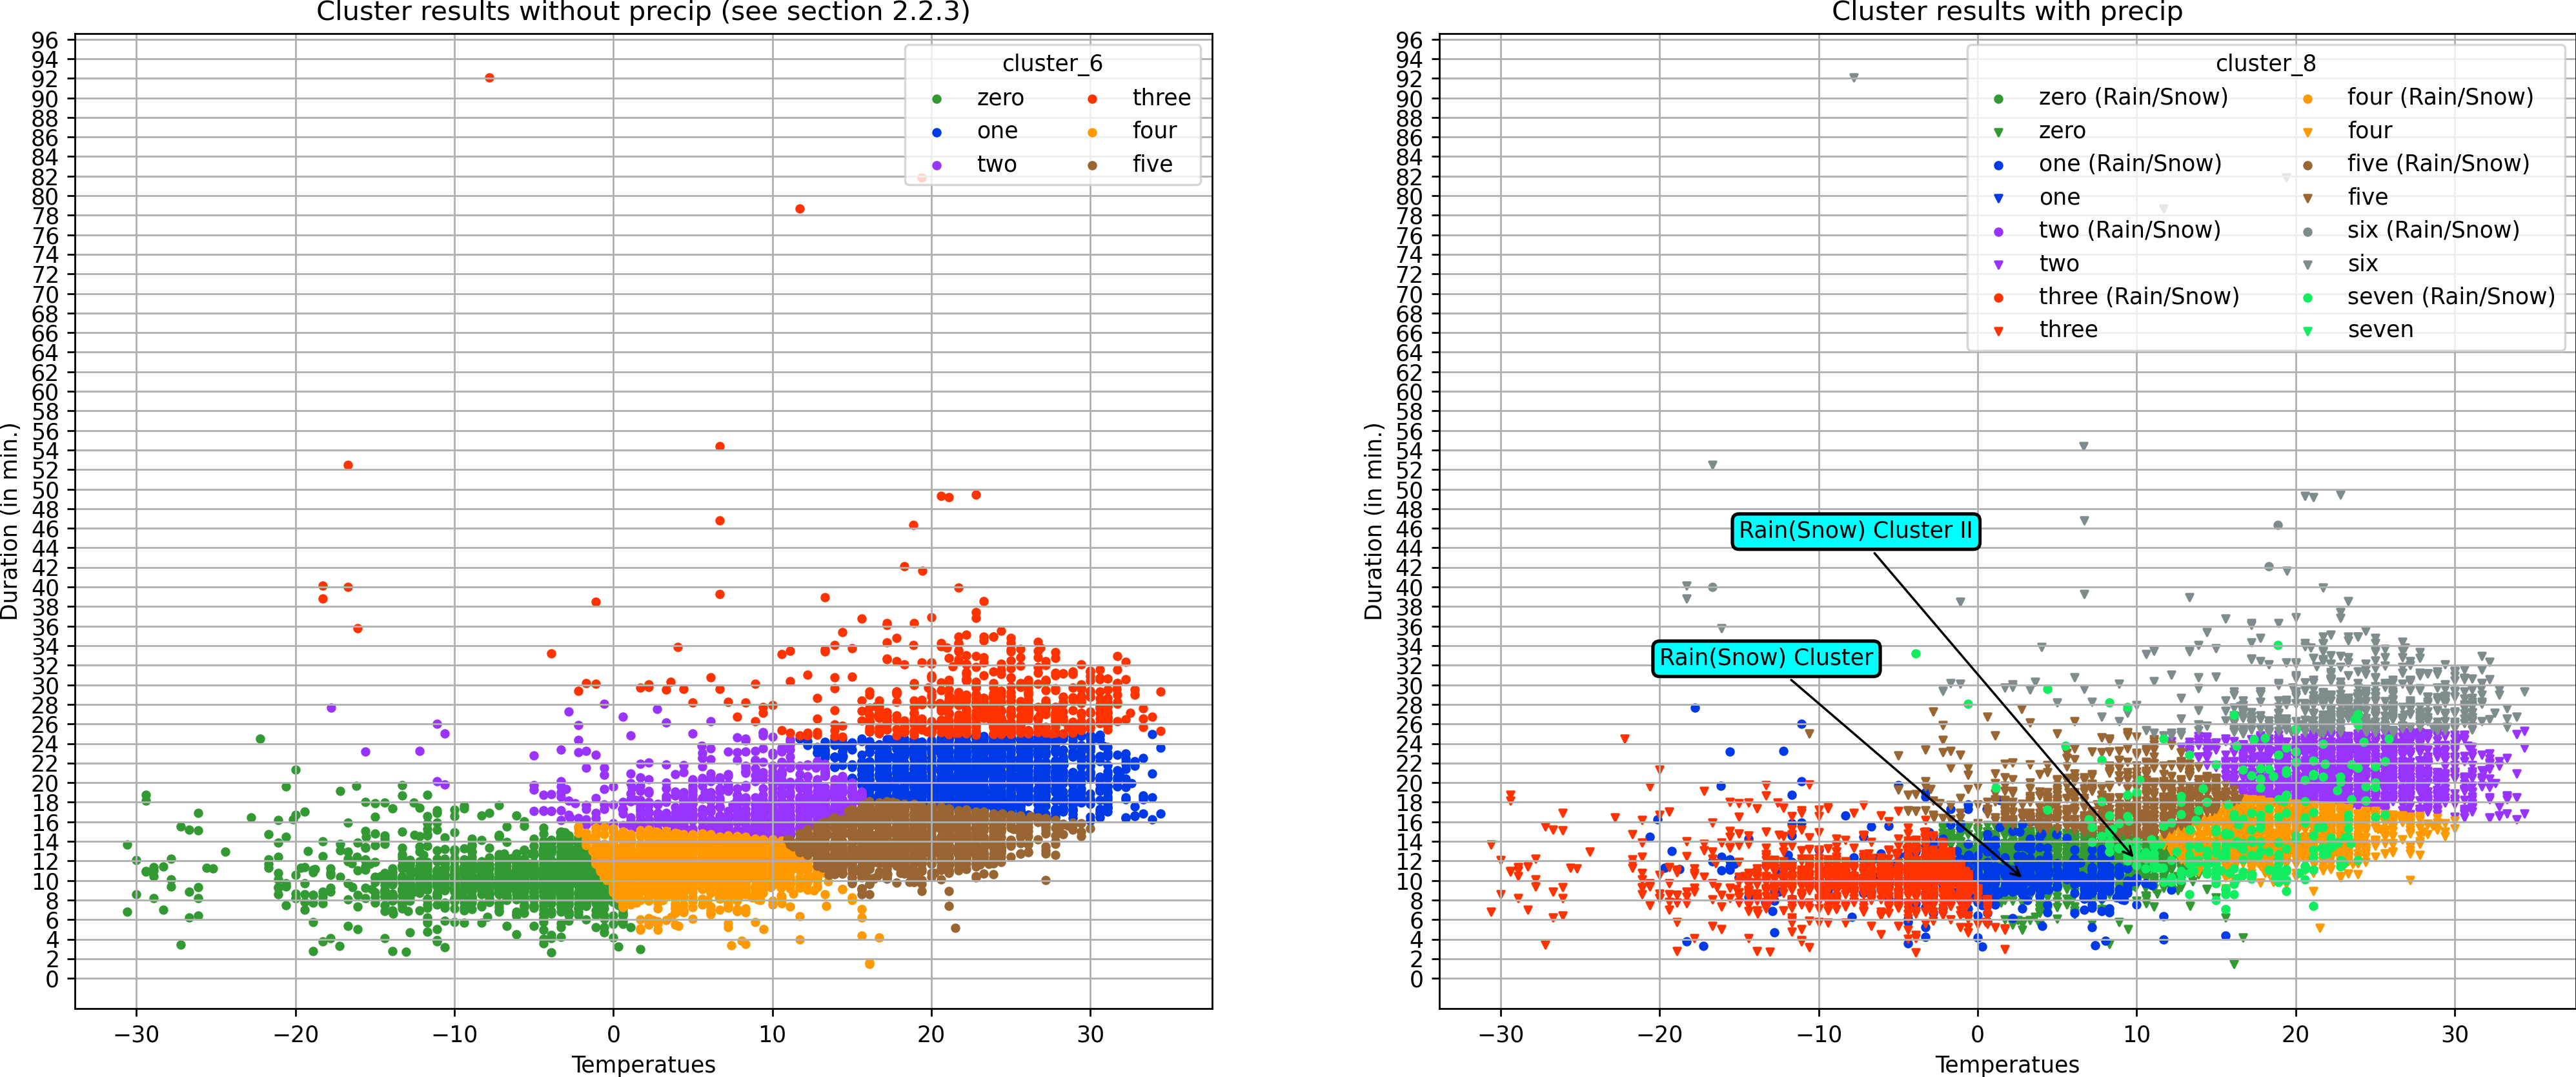
\includegraphics[width=1\linewidth]{./Figures/FINAL_Cluster_Duration_Temp_Precip.png}
    \caption{Cluster result K-Means with and without precip}
    \label{FINAL_Cluster_Duration_Temp_Precip}
\end{figure}

We decided to cluster the revenue hourly (averaged) to yield a reasonable amount of data with K-Means and GMM. The Silhouette Score for the latter one \hyperref[BCABB1]{( Appendix Figure X)} indicates that three clusters are optimal.
The results of the K-Means are found in (\hyperref[BCAPP1]{Appendix X} and \hyperref[BCAPP2]{X}). We found the GMM clusters to be more reasonable, thus we continued to work with those (\hyperref[BCABB2]{Figure X}). 

\begin{figure}[H]
   \centering
    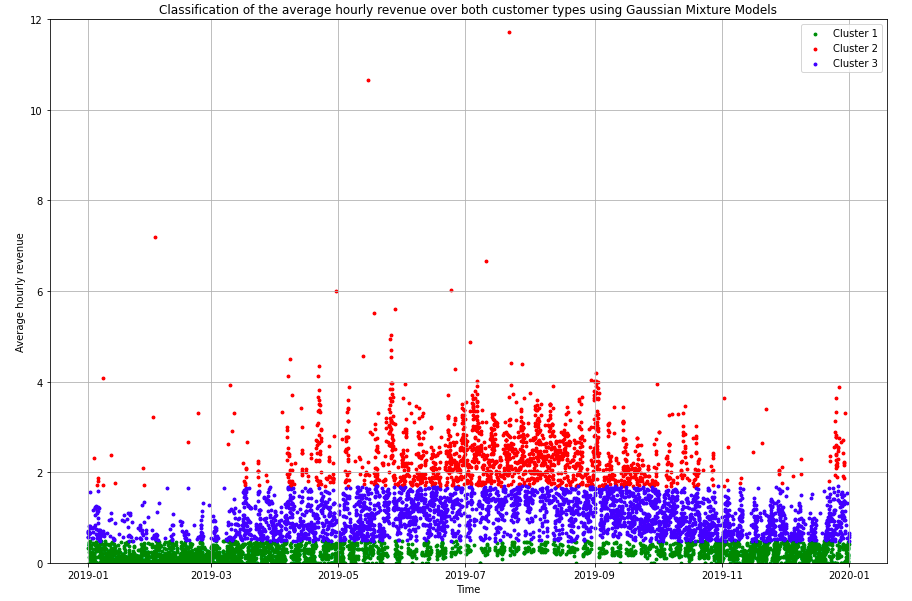
\includegraphics[width=0.8\linewidth]{./Figures/BC_ABB2.png}
    \caption{Classification of the average hourly revenue over both customer types using Gaussian Mixture Models}
    \label{BCABB2}
\end{figure}

Looking at the monthly share of revenue per cluster (\hyperref[BCABB3]{Figure X}), it is evident that during winter, autumn and spring, usually the blue cluster accounts for most of the revenue, although in January and February, the share of the green cluster is nearly equally high. During summer however, especially in July and August, the red cluster accounts for the absolute majority of the revenue, indicating the importance of long rides during the warm summer months for the ride sharing system. Adding the average hourly temperature as input feature does not yield relevant insights, which is described in (\hyperref[BCAPP5]{Appendix X - X}).

\begin{figure}[H]
   \centering
    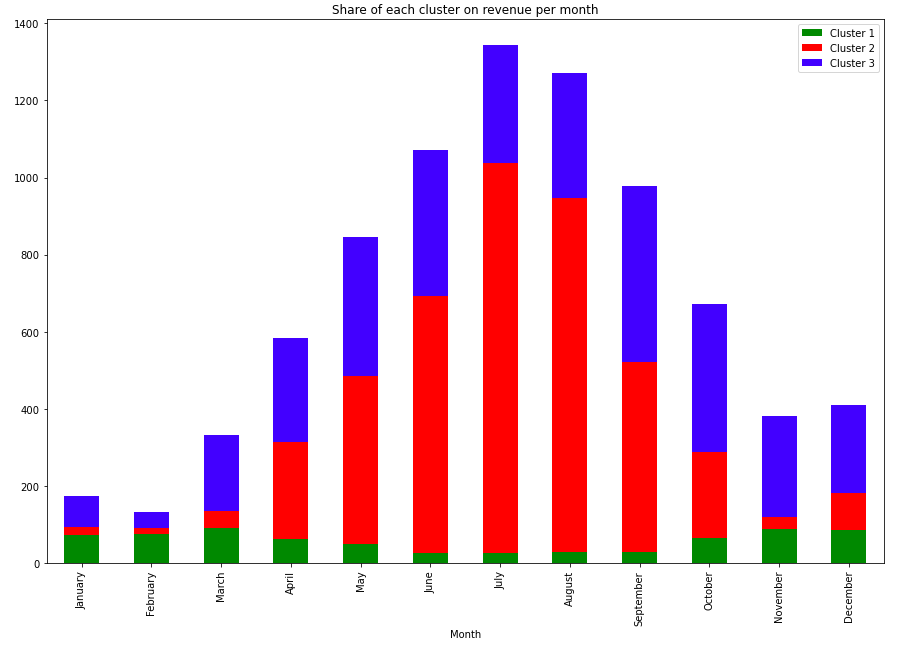
\includegraphics[width=0.65\linewidth]{./Figures/BC_ABB3.png}
    \caption{Share of each cluster on revenue per month}
    \label{BCABB3}
\end{figure}

Now, the individual stations were clustered, beginning with the Demand-Capacity (see the descriptive part for the explanation) as the sole input feature. Applying K-Means and again using the elbow-method (\hyperref[BCABB7]{Appendix Figure X}) does not yield a clear optimal number of clusters, however we discovered a clear three-ring structure in the descriptive analysis and thus chose three clusters. 

\begin{figure}[H]
   \centering
    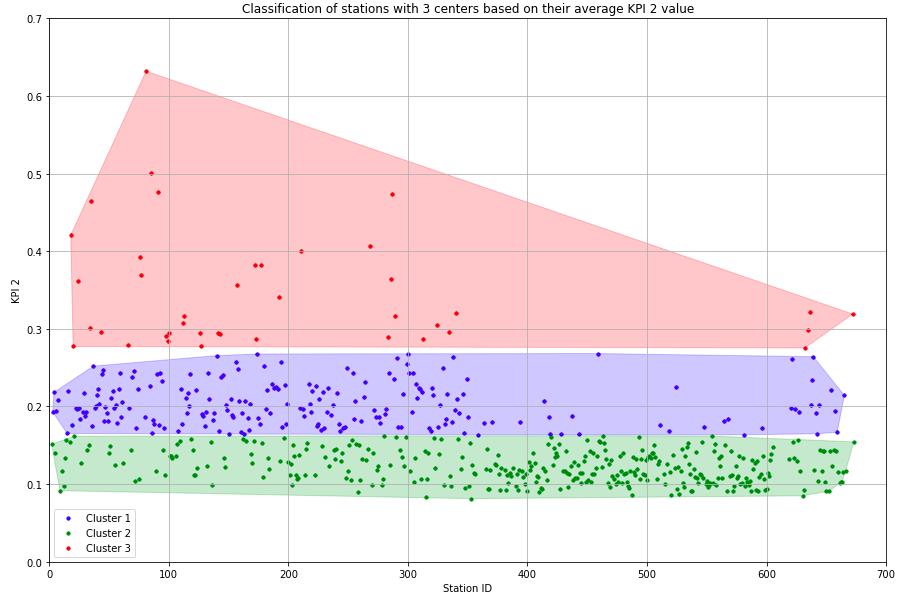
\includegraphics[width=0.8\linewidth]{./Figures/BC_ABB8.png}
    \caption{Classification of stations with 3 centers based on their average KPI2 value}
    \label{BCABB8}
\end{figure}

\begin{figure}[H]
   \centering
    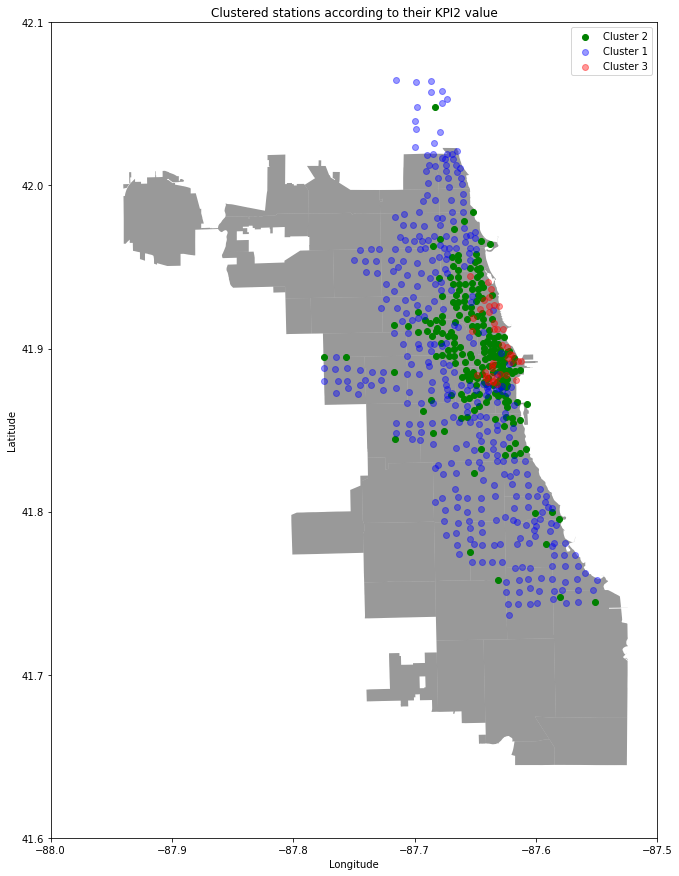
\includegraphics[width=0.75\linewidth]{./Figures/BC_ABB9.png}
    \caption{Clustered stations according to their KPI2 value}
    \label{BCABB9}
\end{figure}

(\hyperref[BCABB8]{Figure X}) illustrates the clusters and serves only as a supporting graph to understand the mapped values (\hyperref[BCABB9]{Figure X}). Here, we can clearly observe the above-mentioned three-ring-structure. Comparing the sketch map in the notebook with a Google Maps representation of Chicago, it gets clear that the majority of the red stations are located near recreational areas close to lake Michigan. A second smaller cluster of red stations seems to be located in downtown/roughly north to the University of Illinois/Chicago. We deduce the following hypothesis: The red stations comprise mainly leisure stations, that are used for recreational purposes. This is backed by the figure in  (\hyperref[BCABB10]{Figure X}), where the “red” Demand-Capacity development is largely season dependent - this makes sense, as during summer, there are obviously more rides related to recreational purposes. The blue and green cluster cannot be significantly distinguished. Several other input features were applied in  (\hyperref[BCAPP8]{Appendix X - X}) without new insights.

\begin{figure}[H]
   \centering
    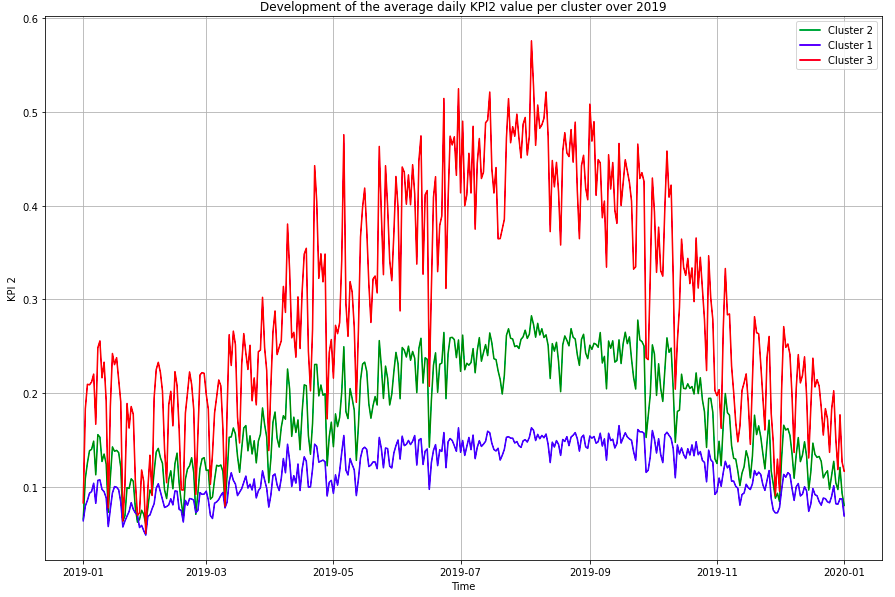
\includegraphics[width=0.7\linewidth]{./Figures/BC_ABB10.png}
    \caption{Development of the average daily KPI2 value per cluster over 2019}
    \label{BCABB10}
\end{figure}

A last insightful clustering using K-Means was created based on the total number of starting rides per station and the average duration of the rides starting there. 4 clusters were found to be suitable (\hyperref[BCABB11]{Appendix Figure X}) and plotting them (\hyperref[BCABB12]{Figure X}) shows, that the red cluster stands out as it exhibits the least proximity to the group of the other three clusters. The yellow and green cluster are relatively similar in terms of their total number of starting rides but seem to show significant differences in terms of the average ride duration starting at the respective stations. When mapping the stations accordingly (\hyperref[BCABB13]{Figure X}), \hyperref[clusterRingsTable]{Table X} summarizes the ring structure.

\begin{figure}[H]
   \centering
    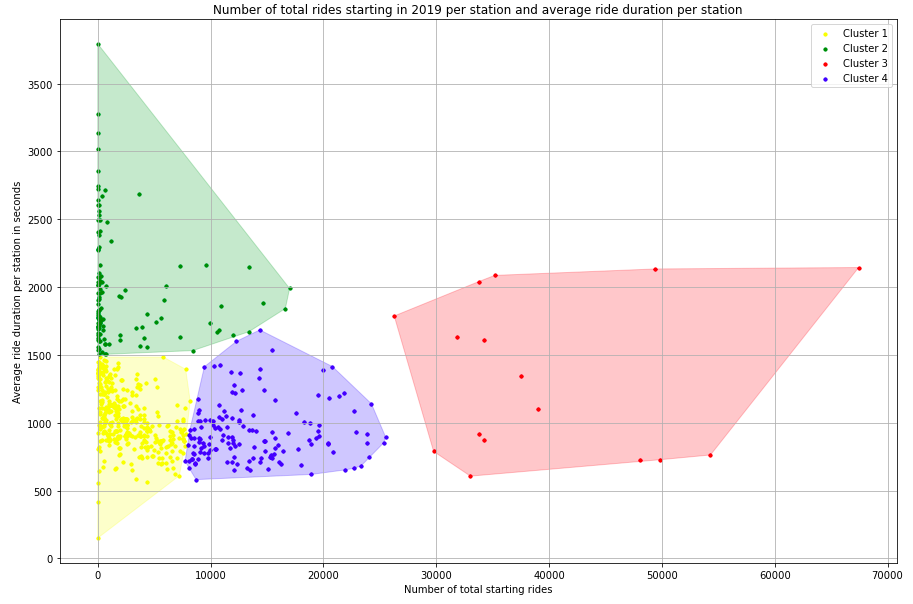
\includegraphics[width=0.8\linewidth]{./Figures/BC_ABB12.png}
    \caption{Number of total rides starting in 2019 per station and average ride duration per station}
    \label{BCABB12}
\end{figure}

\begin{table}[H]
\begin{tabular}{p{0.2\textwidth}p{0.75\textwidth}}
    \toprule
    \textbf{Ring} & \textbf{Description} \\
    \midrule
    Red Cluster & 
    \begin{itemize} 
        \item The red stations are not as predominant as in earlier plots 
        \item They are again mainly located around recreational sites. 
    \end{itemize}\\
    \hline
    Yellow and Green &   \begin{itemize}
        \item The ring comprised by the green and yellow stations exhibits a new structure:
        \item The green stations seem to form a circle around the yellow stations and thus, around the city. 
        \item The green stations seem to form a circle around the yellow stations and thus, around the city. 
        \item Makes sense, as the green stations exhibit roughly the same number of rides as the yellow stations, however they showed a higher average riding duration. 
        \item Thus, the rides from the green outskirt ring seem to be heading towards the center of the city, as their average ride duration is the highest compared to all other clusters
        \item The other clusters do not exhibit this behavior. They might be considered "housing" areas.
    \end{itemize}\\
    \hline
    Blue Cluster & 
    \begin{itemize}
        \item The second ring was also exhibited above
        \item It corresponds to rides roughly as long as the yellow ones
        \item The rides starting there will thus be heading to stations within the blue, red or close yellow stations
    \end{itemize}\\
    \bottomrule
\end{tabular}
\caption{\label{clusterRingsTable}Cluster Rings}
\end{table}


\begin{figure}[H]
   \centering
    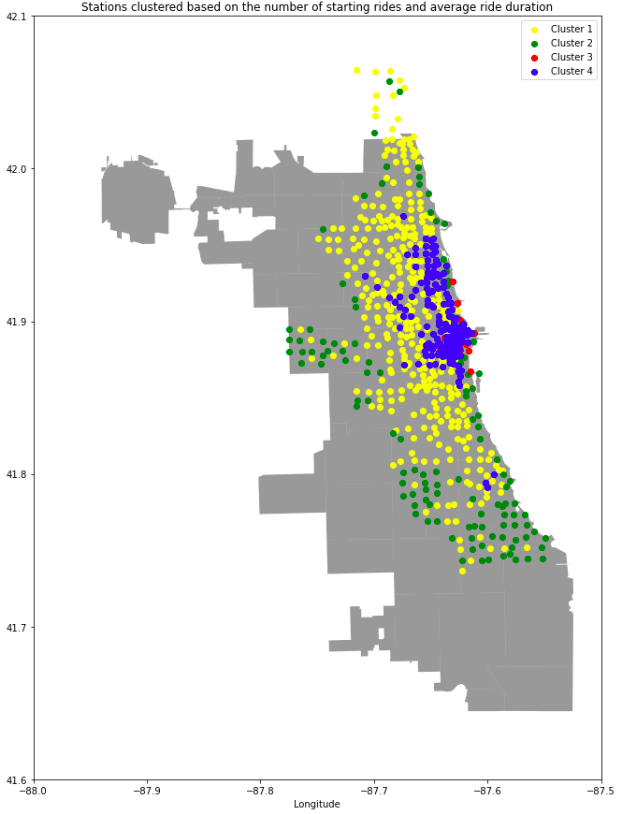
\includegraphics[width=0.8\linewidth]{./Figures/BC_ABB13.png}
    \caption{Stations clustered on the number of starting rides and average ride duration}
    \label{BCABB13}
\end{figure}

\subsection{Predictive Analysis}
\label{subsec:prediction}

As the future demand is a key factor that will guide operational decision-making of Divvy Bikes, total system-level demand in the next hour was forecasted. In order to do that, we developed prediction models with linear regression, random forests and XGBoost. Our features are derived from the dataset \hyperref[Pred_Fig_1]{see Appendix Figure 19}.

We desided to use linear regression models, due to their simplicity and because their use is quasi state-of-the art. While doing so, we immediately faced the problem of missing linearity in our data. Nevertheless, we used Multi-Linear Regression as a first look into regression. Our best model excludes the features ‘season’ and ‘isWeekday’ and reached an r$^{2}$ of roughly 0.6. Because of the missing linearity, we decided to also try Polynomial Regression with the same features, which resulted in strongly improved results. In addition, we also applied both L1 and L2 regularization. In the end, we yield our best Linear/Polynomial Regression model with L1 regularization, with an r$^{2}$ of about 0.9 for the prediction and an MAE around 99.

\begin{figure}[H]
   \centering
    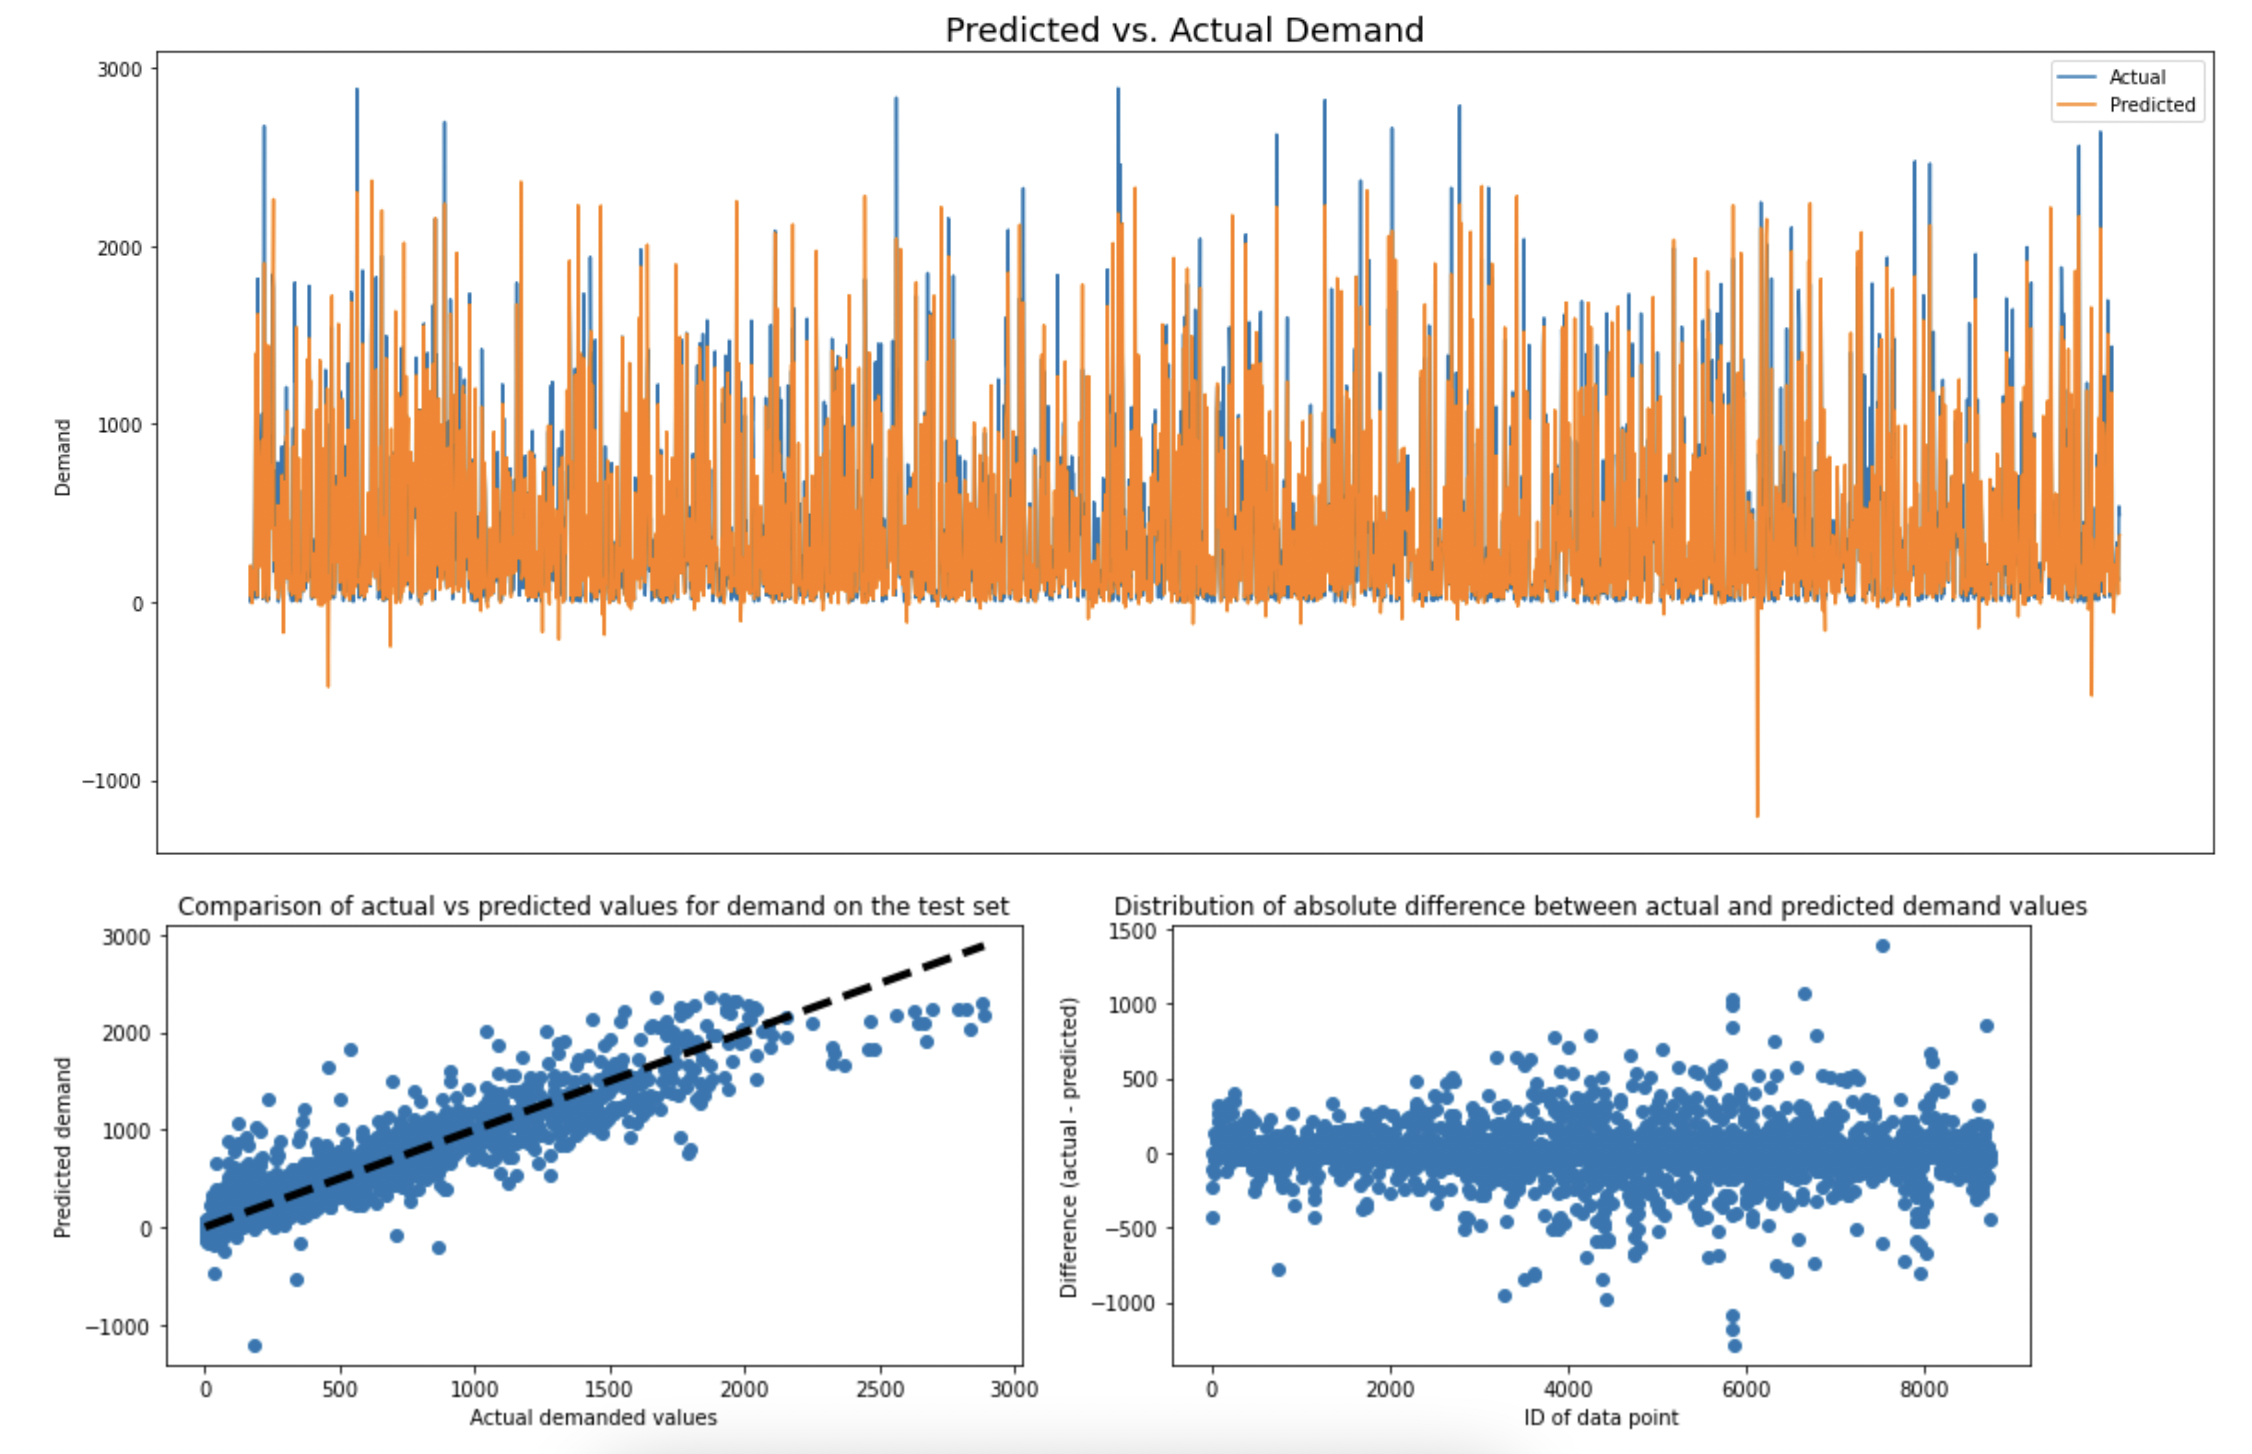
\includegraphics[width=1\linewidth]{./Figures/l1_final.png}
    \caption{Prediction visualization of best L1 model}
    \label{l1}
\end{figure}


For our second and best model, we used the Random Forest algorithm. It is an ensemble method which uses multiple decision trees to make predictions based on a mean computation (in regression) of all trees (see Appendix \hyperref[RF_Intro]{Figure 19} for a visualization). The exact algorithm description and reasons why we chose it as one of our model can be found in the appendix (XXX). To find the best model possible, first a feature selection process was conducted in which different features were selected, and their impact was assessed. Based on their impact on the R2 and MAE and their increase in complexity, the features were then either removed or included in the model. The MAE error metric was used because it has practical relevance, stating that on each hourly prediction x bikes were predicted too much or too less. The R2 error metric describes the proportion of variance in the dependent variable that is accounted for by the model and thus, is also a good measurement of overfitting. The following table illustrates the process. At the end, we decided to select model 5, as model 4 has three more features and is more complex, and the metrics did not differ significantly.
Afterwards, the hyperparameters were tuned and selected. For that, we first looked at the number of estimators (trees in the forest) with cross validation, as can be seen in \hyperref[RF_Fig_1]{Figure 19}. At around 250 estimators, the score does not really change at all, so we picked the number of trees in the forest as 250. To facilitate the hyperparameter tuning and not only focus on one single parameter but on different combinations, we implemented a grid search. Because a whole grid search is computationally heavy, first a random grid search was performed, which limits the possible search space for each optimal parameter. The final results are listed below.
With these values for the hyperparameters, we executed the model on the test set and retrieved an R2 of 91,68 percent.

This means that 91,68 of the proportion of the variance in the demand can be accounted for by the model. The mean absolute error (MAE) is 80,21 which means that in each prediction of the bike demand in one hour, there are 80  too many or too less bikes predicted on average. Benchmarking this, the absolute deviation in the model still seems relatively high, and the Divvy bike provider would still need to maintain 80 additional bikes which are not needed. However, there is a total of more than 6.000 bikes in the Divvy bike fleet, so the prediction error accounts only for about 1 of all bikes which is handleable for the provider. The results of the model are visualized in \hyperref[RF_Fig_2]{Figure 20}. The dashed line would be the optimal prediction line, e.g. if the actual demand is 1.000 the predicted demand would ideally be 1.000 as well. It can be seen that the majority of prediction points reside near the optimal line. In the second figure, the deviations can be inspected more precise. Most of the prediction points lie between -100 and 100 which is as also expressed through the mean absolute error (MAE) of 80. However, some outliers to exist with the extreme of approximately -1.500 demanded bikes on one day.
\begin{figure}[H]
   \centering
    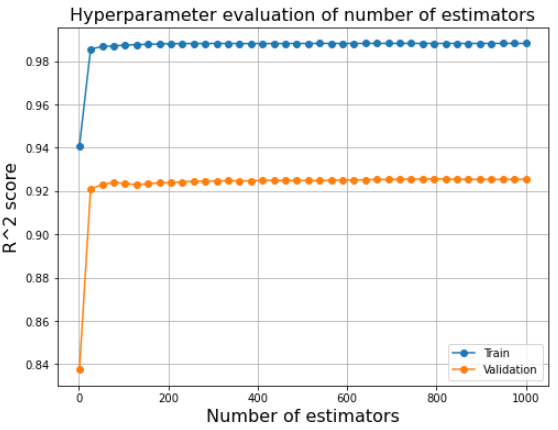
\includegraphics[width=0.5\linewidth]{./Figures/RF_Fig_2.png}
    \caption{Hyperpararmeter evaluation of number of estimators}
    \label{RF_Fig_2}
\end{figure}

\begin{figure}[H]
   \centering
    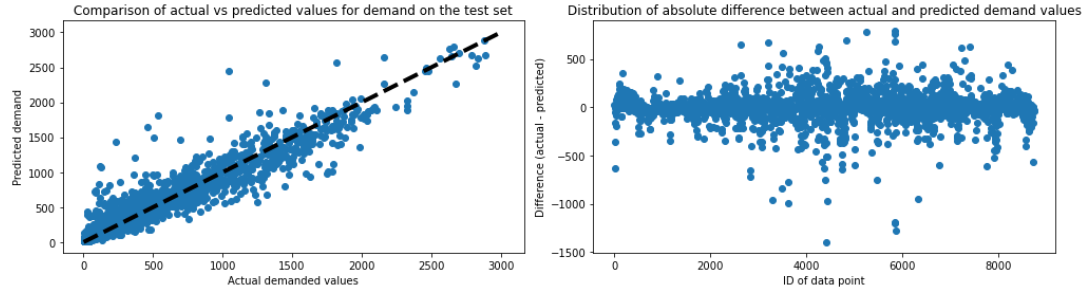
\includegraphics[width=1\linewidth]{./Figures/RF_Fig_3.png}
    \caption{Comparison of actual vs predicted values for demand on the test set and Distribution of absolute difference between actual and predected demand values}
    \label{RF_Fig_3}
\end{figure}
As third regression algorithm we decided to use XGBoost, an ensemble method. The "state-of-the-art” machine learning algorithm can deal well with structured data and is fast, especially compared to other implementations of gradient boosting. The results of the first model are good with a R-squared error of 97 for the train and 92 for validation. Also, the mean absolute error (MAE) and the Root Mean Squared Error (RMSE) indicate that the model is relatively accurate. Using grid search to tune the hyperparameters improved the model, but only slightly resulting in a R-squared error of 93 for the validation.
\begin{figure}[H]
   \centering
    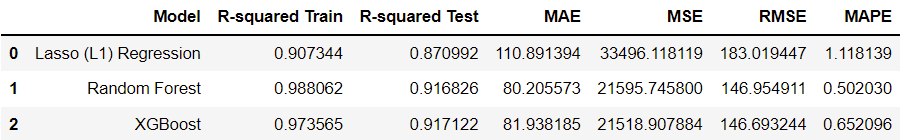
\includegraphics[width=1\linewidth]{./Figures/Predictive_Table_Result.png}
    \caption{Predective analytics results}
    \label{RF_Fig_4}
\end{figure}